\documentclass[11pt]{article}
\usepackage[letterpaper, margin = 1 in]{geometry}
\usepackage{tabularx}
\usepackage{ltablex}
\usepackage{tabularray}
\usepackage{array}
\usepackage{booktabs}
\usepackage{longtable}
\usepackage{caption}
\usepackage{verbatim}
\usepackage{graphicx}
\usepackage{float}
\usepackage{pdflscape}
\usepackage{hyperref}
\usepackage[most]{tcolorbox}

\newtcolorbox{exampleblock}[1][]{
	enhanced,
	breakable,
	boxrule=0pt,
	colback=white,
	left=6pt,
	borderline west={2pt}{0pt}{#1}
}


\title{\textbf{Revision 0: \\Validation and Verification \\ \large Group 8 - C.A.V.E: Cave Assessment and Visualization Equipment}}
\author{Abdul Rahim Khan \\ Andrew Brink \\ Gokberk Yilmaz \\ Nicholas Trimble \\ Tabish Faisal}
\date{February 10, 2026}

\begin{document}
	
	\maketitle
	~\newpage
	\pagenumbering{roman}
	\renewcommand{\thetable}{\Roman{table}}
	\setcounter{table}{0}
	\begin{table}[hp]
		\caption{Revision History} \label{TblRevisionHistory}
		\begin{tabularx}{\textwidth}{llX}
			\toprule
			\textbf{Date} & \textbf{Developer(s)} & \textbf{Change}\\
			\midrule
			February 1, 2026 & All Members & Initial Draft\\
			\midrule
			February 10, 2026 & All Members & Finished Document\\
			\bottomrule
		\end{tabularx}
	\end{table}
	
	~\newpage
	\section*{Glossary}
		\setcounter{table}{1}
	\begin{table}[hp]
		\centering
		\begin{tabularx}{\textwidth}{X p{0.6\textwidth}}
			\toprule
			\textbf{Term} & \textbf{Definition} \\
			\midrule
			IMU & Inertial measurement unit, providing acceleration and rotational data \\
			\addlinespace
			LiDAR & Light Detection and Ranging: a sensor that uses a rotating laser to measure distances to objects. \\
			\addlinespace
			Point cloud & A collection of coordinate points in 3D space \\
			\addlinespace
			Portable device & The portion of the design that is carried with the user/operator for mapping an enclosed space \\
			\addlinespace
			TOF sensor & Time of Flight sensor, which uses pulses of infrared light and a sensor that measures the time at which the light is received back to create a point cloud. \\
			\addlinespace
			ICP & Iterative closest point algorithm minimizes the differences between subsequent point clouds to reconstruct 3D surfaces. \\
			\bottomrule
			\caption{Terms and definitions}
		\end{tabularx}
	\end{table}
	~\newpage
	
	{
		\hypersetup{pdfborder = {0 0 0}}
		\tableofcontents
		\listoffigures
		\listoftables
	}
	
	\cleardoublepage
	\renewcommand{\thetable}{\arabic{table}}
	\setcounter{table}{0}
	
	\section{Introduction}
	\pagenumbering{arabic}
	\subsection{Purpose}
	
	The purpose of this document is to validate and verify that the project requirements are feasible and achieve the objectives laid out in the contract. This serves as a checkpoint in the development process where we assess whether our software and hardware are capable of fulfilling the project requirements. The verification process provides a set of pass/fail tests which the current revision is tested against to determine requirement completion.
	
	\subsection{Scope}
	This validation and verification encompass the entire C.A.V.E. design, including software, electrical, and mechanical components. Requirements are defined in \href{https://github.com/4tb6-cave/capstone/blob/main/docs/HazardAnalysis/HazardAnalysis.pdf}{Revision 0: Requirements and Hazard Analysis}. The scope covers all the behavioural, timing, and software/hardware requirements tied the system. Additionally, this document addresses the modifications to the original requirements based on the implementation experience and feasibility checks conducted during the validation process.
	
	\section{Validation} 
	
	%**Natural language evaluation of the requirements, how well they meet the objectives, what the user interface is like. Validates that the hardware/design we have chosen is capable of meeting the requirements 
	The validation process examines each requirement through a qualitative metric, assessing whether our system design choices fulfill and support the overall project objectives.
	
	
	\subsection{Behavioural Requirements} 
	
	\subsubsection{RB1} 
	
	\begin{exampleblock}
		The device will produce a point cloud C\_point\_cloud representing the physical surfaces mapped by the sensors (M\_tof\_data, M\_imu\_gyro) while recording is enabled (M\_start\_stop == true).
	\end{exampleblock}
	
	The C.A.V.E system achieves this fundamental requirement by fusing the data from multiple sensors: the ToF sensors actively (M\_start\_stop == true) provides the point cloud (M\_tof\_data) at each consecutive time-stamps while the IMU outputs orientation and rotational data (M\_imu\_gyro) that allows the system to properly map out successive point cloud in a 3D global space.
	
	The oriented point clouds are now passed through our ICP algorithm which further refines the reconstruction of the scanned environment by aligning the consecutive point cloud frames, minimizing the distance between each capture and producing a coherent and recognizable final point cloud (C\_point\_cloud).
	
	\subsubsection{RB2 (Removed)}
	 
	\begin{exampleblock}[red]
		The confidence in the accuracy of C\_point\_cloud shall be represented by C\_confidence.
	\end{exampleblock}
	
	In the process of designing and implementing the algorithms for fusing the sensor data, we have concluded that this requirement is not necessary for the fulfillment of our goal. Providing a metric for the confidence of the system has proved to be a difficult task and is not required to achieve the primary goal, which is to produce the point cloud. Our implementation either succeeds in fusing the data, or it fails to do so because of an error, but there is no intermediate state where the model is 50\% correct. 
	
	We considered replacing this requirement with a specification that the final point cloud needs to be accurate to the actual cave within a certain threshold, but there are a couple of issues with this. This would be practically the same as the first requirement. However, it would additionally include  error threshold numbers which we would have to arbitrarily decide. Testing this requirement would be impossible without additional expensive equipment like 3D LiDAR. Instead of adding this type or requirement, we decided that our testing for accuracy will have to be qualitative rather than quantitative, and that checking that the features of the model are easily recognizable will be our most important test. This conclusion was based on discussions with Dr. Wassyng. 
	
	\subsubsection{RB3} 
	
	\begin{exampleblock}
		C\_record\_status toggles between indicating recording and standby when M\_start\_stop is toggled by the user. If the system encounters an error it cannot recover from, it must display an error status on C\_record\_status.
	\end{exampleblock}
	
	Completion of this requirement happens via the RPi Head ‘hat’ board on the Raspberry Pi. System software reacts to the pressing of Button 1 to transition from standby to recording. The LED U10 indicates that the system is actively recording the environment, and once Button 1 is pressed again this LED deactivates. Communicating and error on C\_record\_status is achieved by illuminating LED1 “Sensing Error”. This requirement remains the same as the original specification, though the design of the buttons could be difficult to reach or differentiate when the Pi is mounted at the back of the helmet. Additionally, the LEDs may be difficult see by the person wearing the device, however this can be mitigated by operating with another person as a duo, a standard caving safety practice. 
	
	\subsubsection{RB4} 
	
	\begin{exampleblock}
		C\_record\_time will display remaining available recording time by taking the minimum of M\_SOC/const\_power\_rate and M\_storage\_left/const\_datarate.
	\end{exampleblock}
	
	%Recording time, representing storage or battery remaining 
	The Raspberry Pi is powered through a portable powerbank which has a seven-segment display showing the remaining battery percentage. This can be used to calculate the time remaining (C\_record\_time) for the data recording process.
	
	\subsubsection{RB5 (Modified)} 
	
	\begin{exampleblock}[orange]
		Updated: The quality of the point cloud produced by the system must be independent of all external light.
	\end{exampleblock}
	
	Our 5th behavioural requirement previously was that the confidence level had to remain above a certain value when the system was operating in little to no light conditions. However, since the confidence level is no longer being used (see the discussion for RB2), this requirement needs to be altered. The reason for this requirement originally was to ensure that the system would operate properly in the dark conditions of a cave. In keeping with the original intent, we have modified this requirement to remove the mention of C\_confidence. 
	
	This requirement means that all the sensors used should not be sensitive to the lack of natural light and should not be affected by any flashlights being used by the operator. The fulfilment of this requirement is possible because TOF sensors produce their own light, which is in the infrared range. 
	
	
	\subsection{Timing}
	
	\subsubsection{RT1}
	
	\begin{exampleblock}
		Const\_capt\_rate shall be frequent enough to produce complete maps of an environment at a walking pace (3-5km/h)
	\end{exampleblock}
	
	The rate of capture should not be so slow that the operator has to slow down significantly to allow it to function properly. At the same time, there is no need 
	to capture more data than necessary. If the system captures enough data to reconstruct the scene when the operator is walking, that should provide a good balance 
	of these two factors.
	
	\subsubsection{RT2}
	
	\begin{exampleblock}
		Const\_capt\_rate shall be low enough such that the system can complete a measurement of all sensor data before the next interval.
	\end{exampleblock}
	% Need more elaboration with respect to the requirements
	
	Rotating the point clouds with the IMU data produces coherent results. This sensor fusion results in a 3D model that is easy to parse with simple visualization software. We were able to run the ToF and IMU sensors simultaneously to map a small room accurately. 
	
	
	\subsection{Hardware/Software Environment: }
	
	\subsubsection{RE1}  
	
	\begin{exampleblock}
		The portable device shall not require an active internet connection to achieve the behavioural requirements RBX.
	\end{exampleblock}
	
	The device does not need to be connected to any form of internet or Bluetooth and is still able to run completely without hinderance. This can be shown by running the system without it connected to any form of internet or cellular device. 
	
	\subsubsection{RE2} 
	
	\begin{exampleblock}
		The hardware should minimize encumbrance of the user to ensure exploration is not inhibited.
	\end{exampleblock}
	
	The entire device weighs less than two kilograms, as well as having a low profile, which mitigates any form of hinderance to the user it can cause.
	
	
	\section{Verification}
	
	%**Hard set of tests to check the requirements meet a certain level of performance. All tests must either pass or fail based on a threshold 
	In this section, the verification process establishes objective tests with a pass/fail criteria that determine whether each requirement has been successfully implemented in the current system revision. Images for the tests are provided in Appendix A.
	
	\subsection{Behavioural Requirements} 
	
	Several of these tests are well defined, such as those related to the hardware, but some of the algorithm performance metrics are more difficult to define and as mentioned above the requirements have been modified. At the current state of the project, several failures are expected, as much of the device/interface integration remains to be completed. 
	
	\begin{tabularx}{\textwidth}{X p{0.25\textwidth} p{0.2\textwidth} X p{0.2\textwidth}}
		\toprule
		\textbf{Test} & \textbf{Procedure} & \textbf{Expected Result} & \textbf{Pass/Fail} & \textbf{Notes}
		\\
		\midrule
		T-RB1-0 & Record data from ToF and IMU. Fuse data and pass oriented through ICP algorithm which outputs final point cloud. & Point cloud where the environment/scene can be easily recognized & Fail & Scan is not easily recognizable, although the results show some promise. See figures in appendix.
		\\
		\midrule
		T-RB1-1 & Record data from ToF and IMU on to Raspberry Pi for duration of 10 minutes & Data is successfully recorded and no data is lost & Fail & USB errors in TOF sensor communication cause recording to fail after about 1 minute
		\\
		\midrule
		T-RB2-0 & - & - & - & Requirement removed 
		\\
		\midrule
		T-RB3-0 & Press button 1 after system power on & U7, U10 illuminates; recording starts & Fail & U7 illuminates, U10 and recording pending software integration. Button press recognized.
		\\
		\midrule
		T-RB3-1 & Press button 2 after system power on & U8 illuminates & Pass & No software interaction yet. LED overly bright 
		\\
		\midrule
		T-RB4-0 & & & &
		\\
		\midrule
		T-RB5-0 & Use TOF sensor with the same scene in good lighting and poor lighting conditions & All point clouds produced are practically identical & Pass & See pictures of test in appendix \\
		\bottomrule
		\caption{Verification Tests for Behavioural Requirements}
	\end{tabularx}
	
	
	\subsection{Timing} 
	
	Both IMU and ToF data come with timestamps. Using these timestamps, we can ensure both are within 100ms of each other. In our previous tests, we achieved a precision of around 50ms, which is more than enough for a walking pace. 
	
	To further improve this, we can switch to the Linux RT kernel which will make it easier for us to manage the real-time aspect of this project. The Linux RT API allows us to set deadlines for tasks, which would be essential if we need better precision. 
	
	\subsection{Hardware / Software Environment}
	
	The tests are very empirical and easy to determine. To test whether or not the system can run without internet we will run the same program both connected to the internet, and not connected to the internet, and it is expected that there will be no change in the result (as it is not internet dependent). The hardware environment is a bit harder to directly test due to variability, but the system is lightweight and has a small enough footprint it shouldn't hinder mobility. This could be tested by having the user traverse an area without the equipment, and with, and have weighted scaling to determine how much of a hinderance it is. \\
	
	\begin{tabularx}{\textwidth}{X p{0.25\textwidth} p{0.2\textwidth} X p{0.2\textwidth}}
		\toprule
		\textbf{Test} & \textbf{Procedure} & \textbf{Expected Result} & \textbf{Pass/Fail} & \textbf{Notes} \\
		\midrule
		T-RE1-0 & Capture the same arbitrary data with and without an internet connection & Both rosbags should have the same raw information, accounting for general noise & Pass & None\\
		\midrule
		T-RE1-1 & Run the ICP algorithm on the same initial data with and without an internet connection & The ICP should have similar results on both runs, accounting for variability in the algorithm & Pass & None \\
		\midrule
		T-RE2-0 & Measure the overall weight of the design & The entire system should be under 2 kg & Pass & Total Mass of all components is around 0.5-0.7 kg: Helmet, Raspberry Pi, Sensors \\
		\midrule
		T-RE2-1 & Traverse a fixed location at a fixed path with and without the equipment & It should feel the exact same with and without everything worn, or at least not hinder mobility by a good margin & - & This is difficult to empirically decide due to it being opinionated and different for other users, but a general gist is needed. \\
		\bottomrule
		\caption{Verification Tests for Hardware/Software Requirements}
	\end{tabularx}
	
	\newpage
	\section{Appendix A: Verification Test Images}
	
	\begin{figure}[H]
		\centering
		\begin{minipage}{0.48\textwidth}
			\centering
			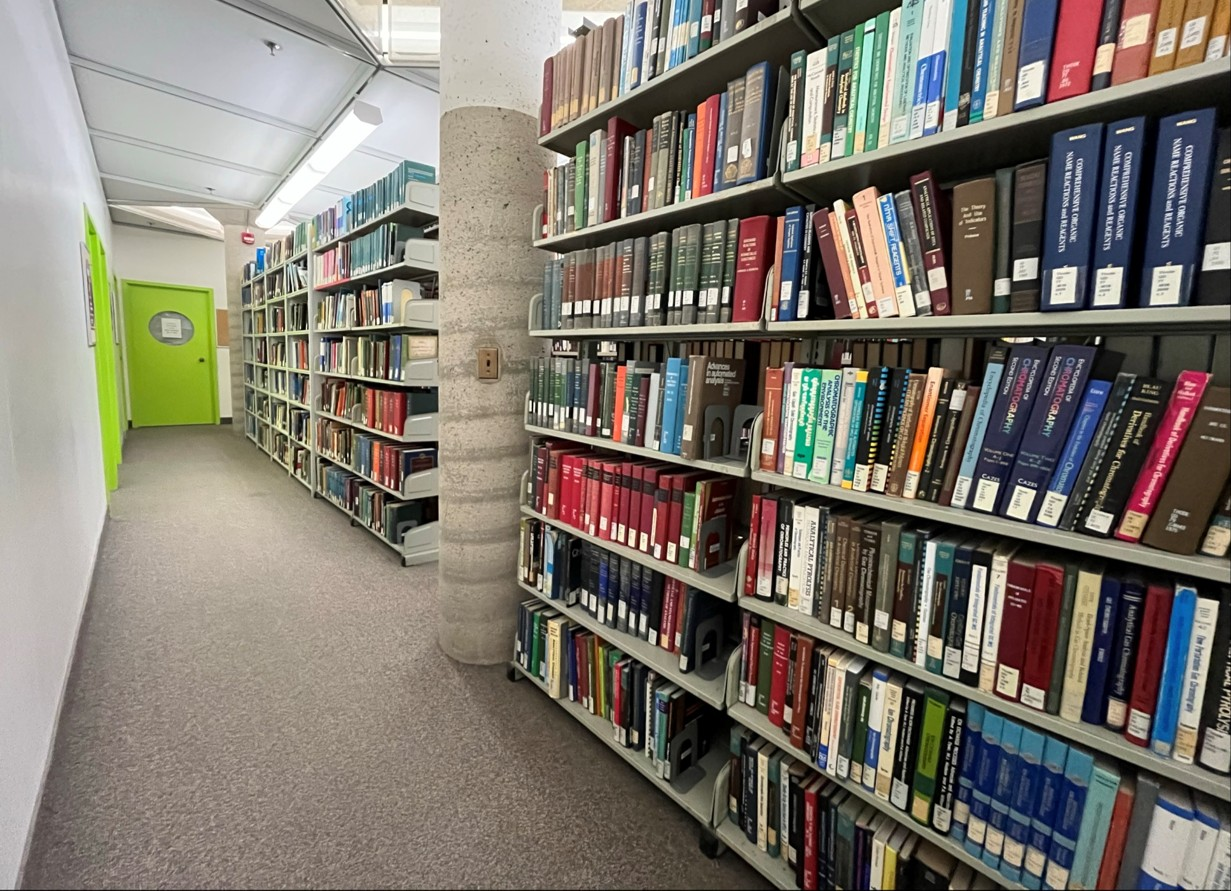
\includegraphics[width=\textwidth]{Images/Test_RB1_pic.jpg}
			\caption*{(a) Test T-RB1-0 (Environment)}
		\end{minipage}\hfill
		\begin{minipage}{0.48\textwidth}
			\centering
			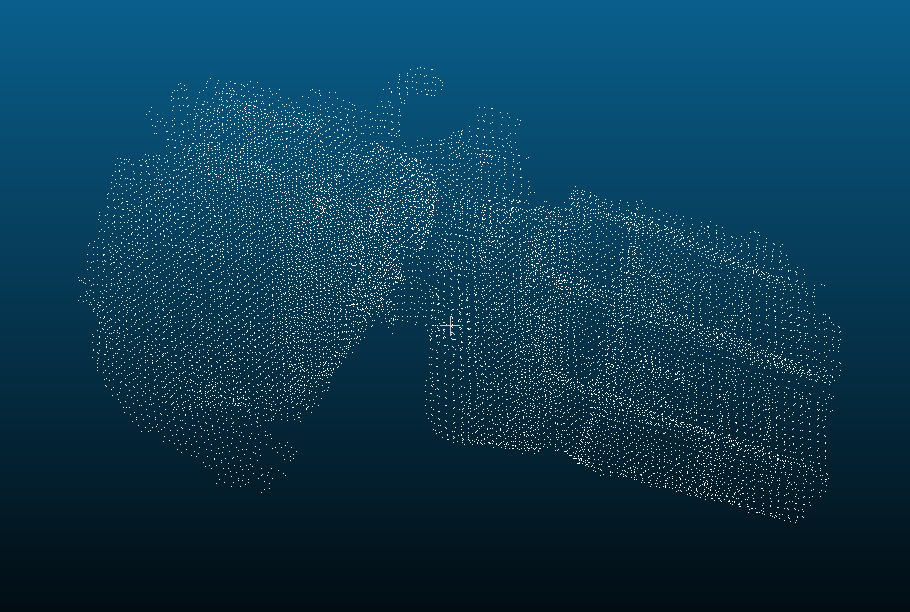
\includegraphics[width=\textwidth]{Images/Test_RB1_icp.png}
			\caption*{(b) Test T-RB1-0 (Output of ICP algorithm)}
		\end{minipage}
		\caption{Test T-RB1-0}
	\end{figure}

	\begin{figure}[H]
		\centering
		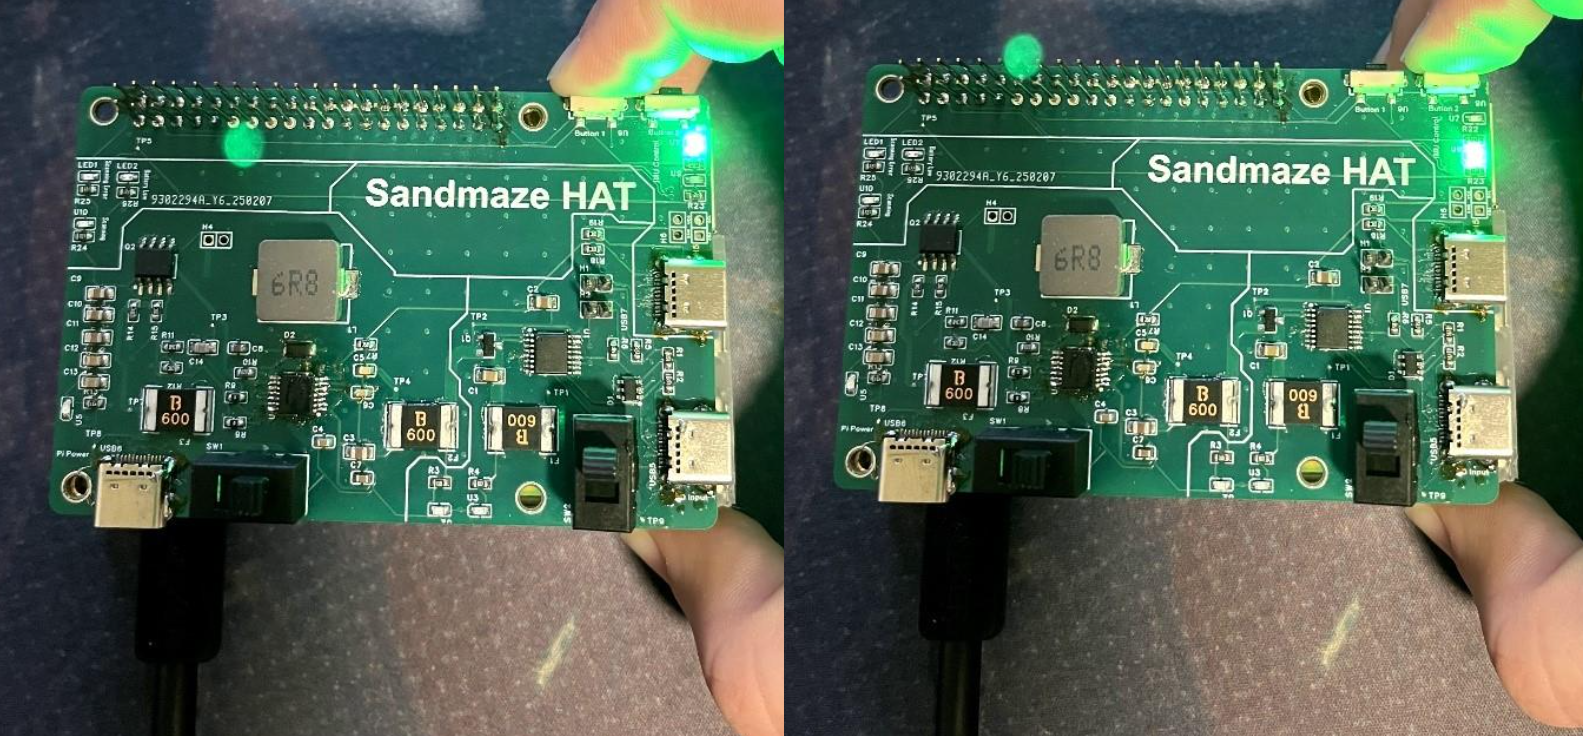
\includegraphics[width=0.75\textwidth]{Images/Test_RB3}
		\caption{Test T-RB3-0/1}
	\end{figure}

	\begin{figure}[H]
		\centering
		\begin{minipage}{0.48\textwidth}
			\centering
			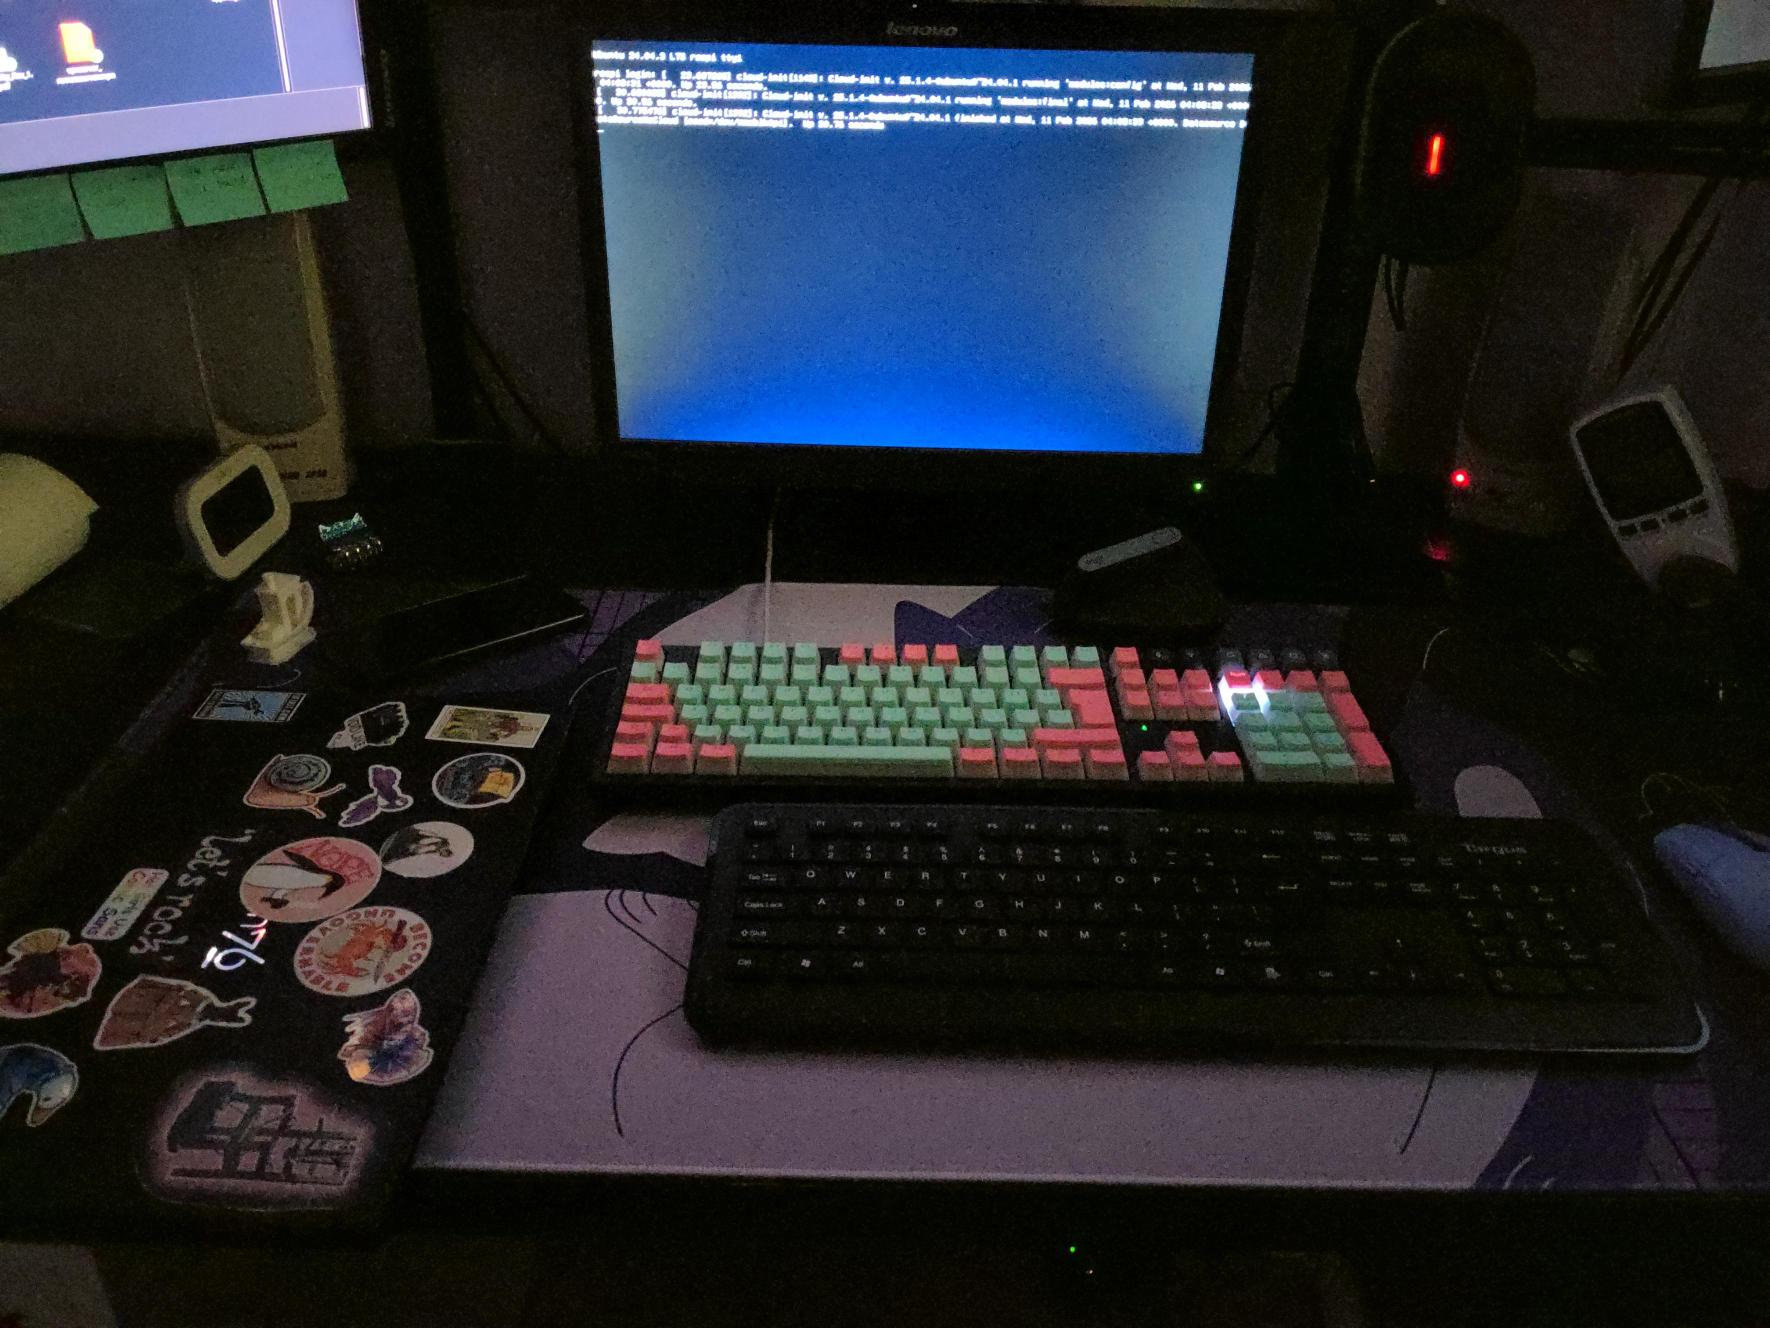
\includegraphics[width=\textwidth]{Images/Test_RB5_dark_pic}
			\caption*{(a) Test T-RB5-0 (Dark environment)}
		\end{minipage}\hfill
		\begin{minipage}{0.48\textwidth}
			\centering
			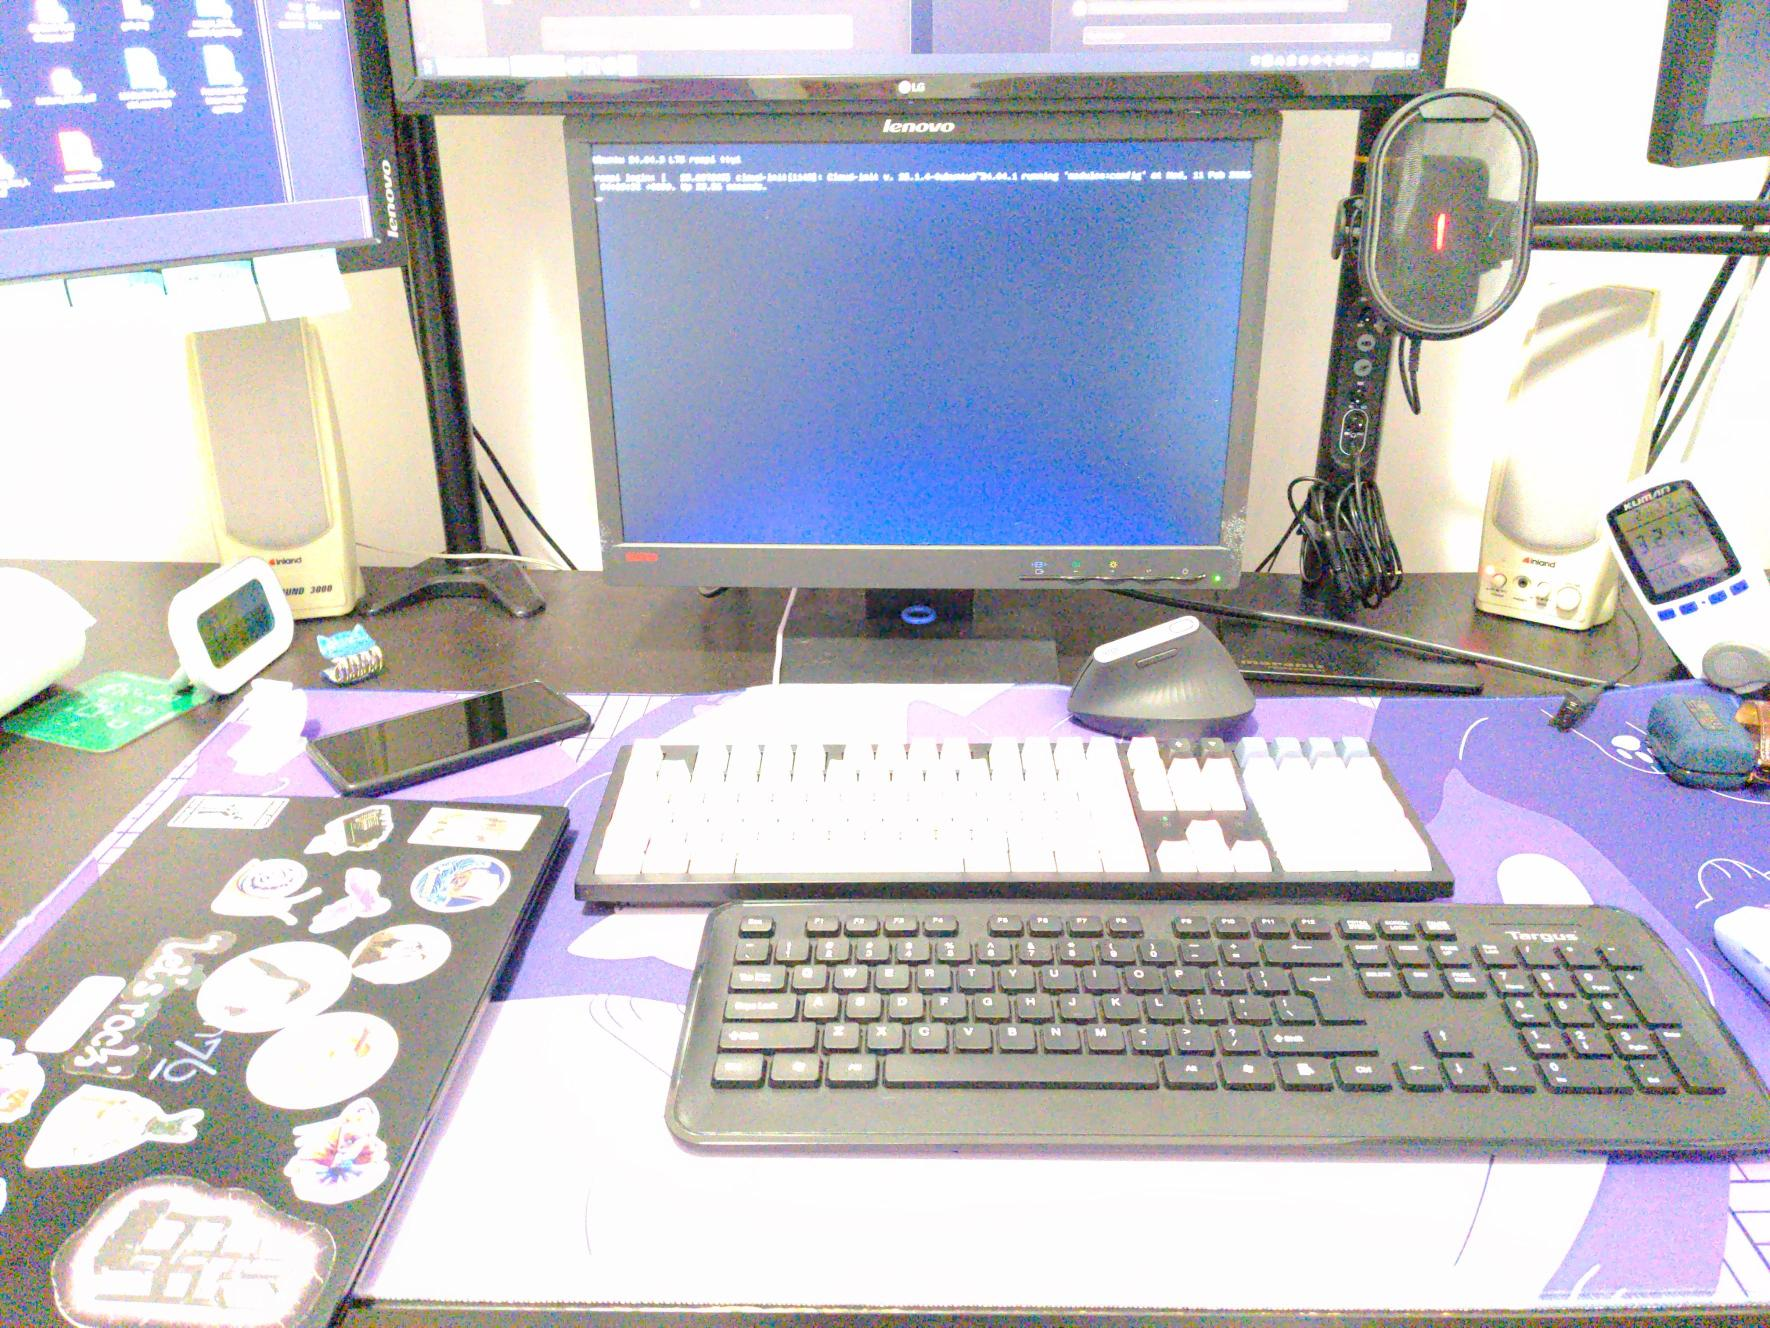
\includegraphics[width=\textwidth]{Images/Test_RB5_light_pic}
			\caption*{(b) Test T-RB5-0 (Light environment)}
		\end{minipage}
		\begin{minipage}{0.48\textwidth}
			\centering
			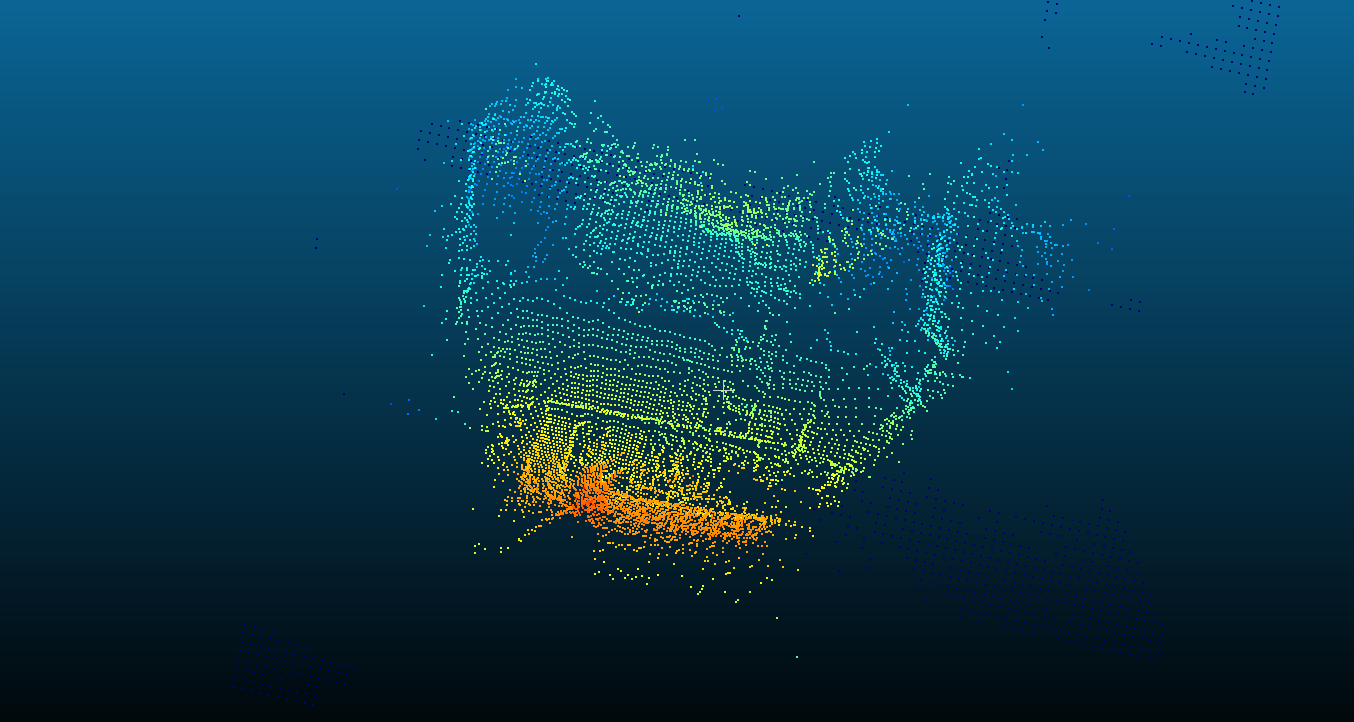
\includegraphics[width=\textwidth]{Images/Test_RB5_dark_tof}
			\caption*{(c) Test T-RB5-0 (Dark TOF capture)}
		\end{minipage}\hfill
		\begin{minipage}{0.48\textwidth}
			\centering
			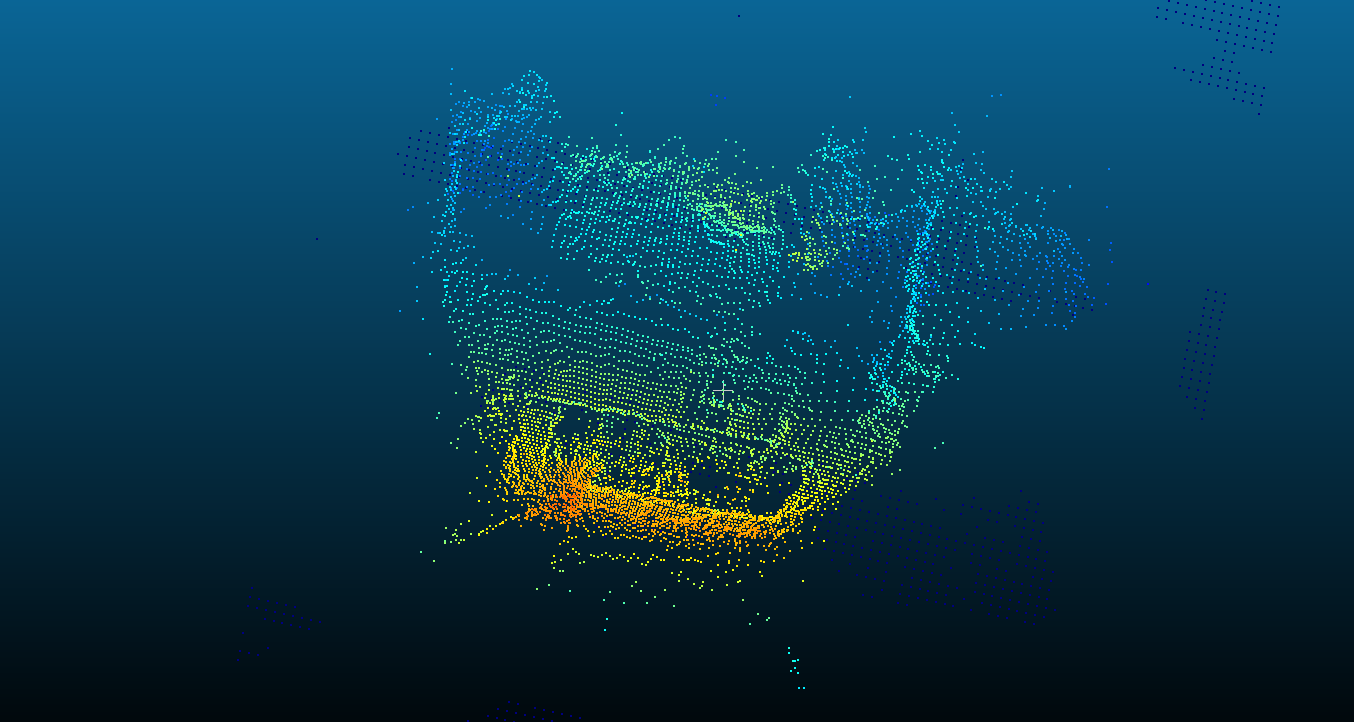
\includegraphics[width=\textwidth]{Images/Test_RB5_light_tof}
			\caption*{(d) Test T-RB5-0 (Light TOF capture)}
		\end{minipage}
		\caption{Test T-RB5-0}
	\end{figure}
	
	\begin{figure}[H]
		\centering
		\begin{minipage}{0.48\textwidth}
			\centering
			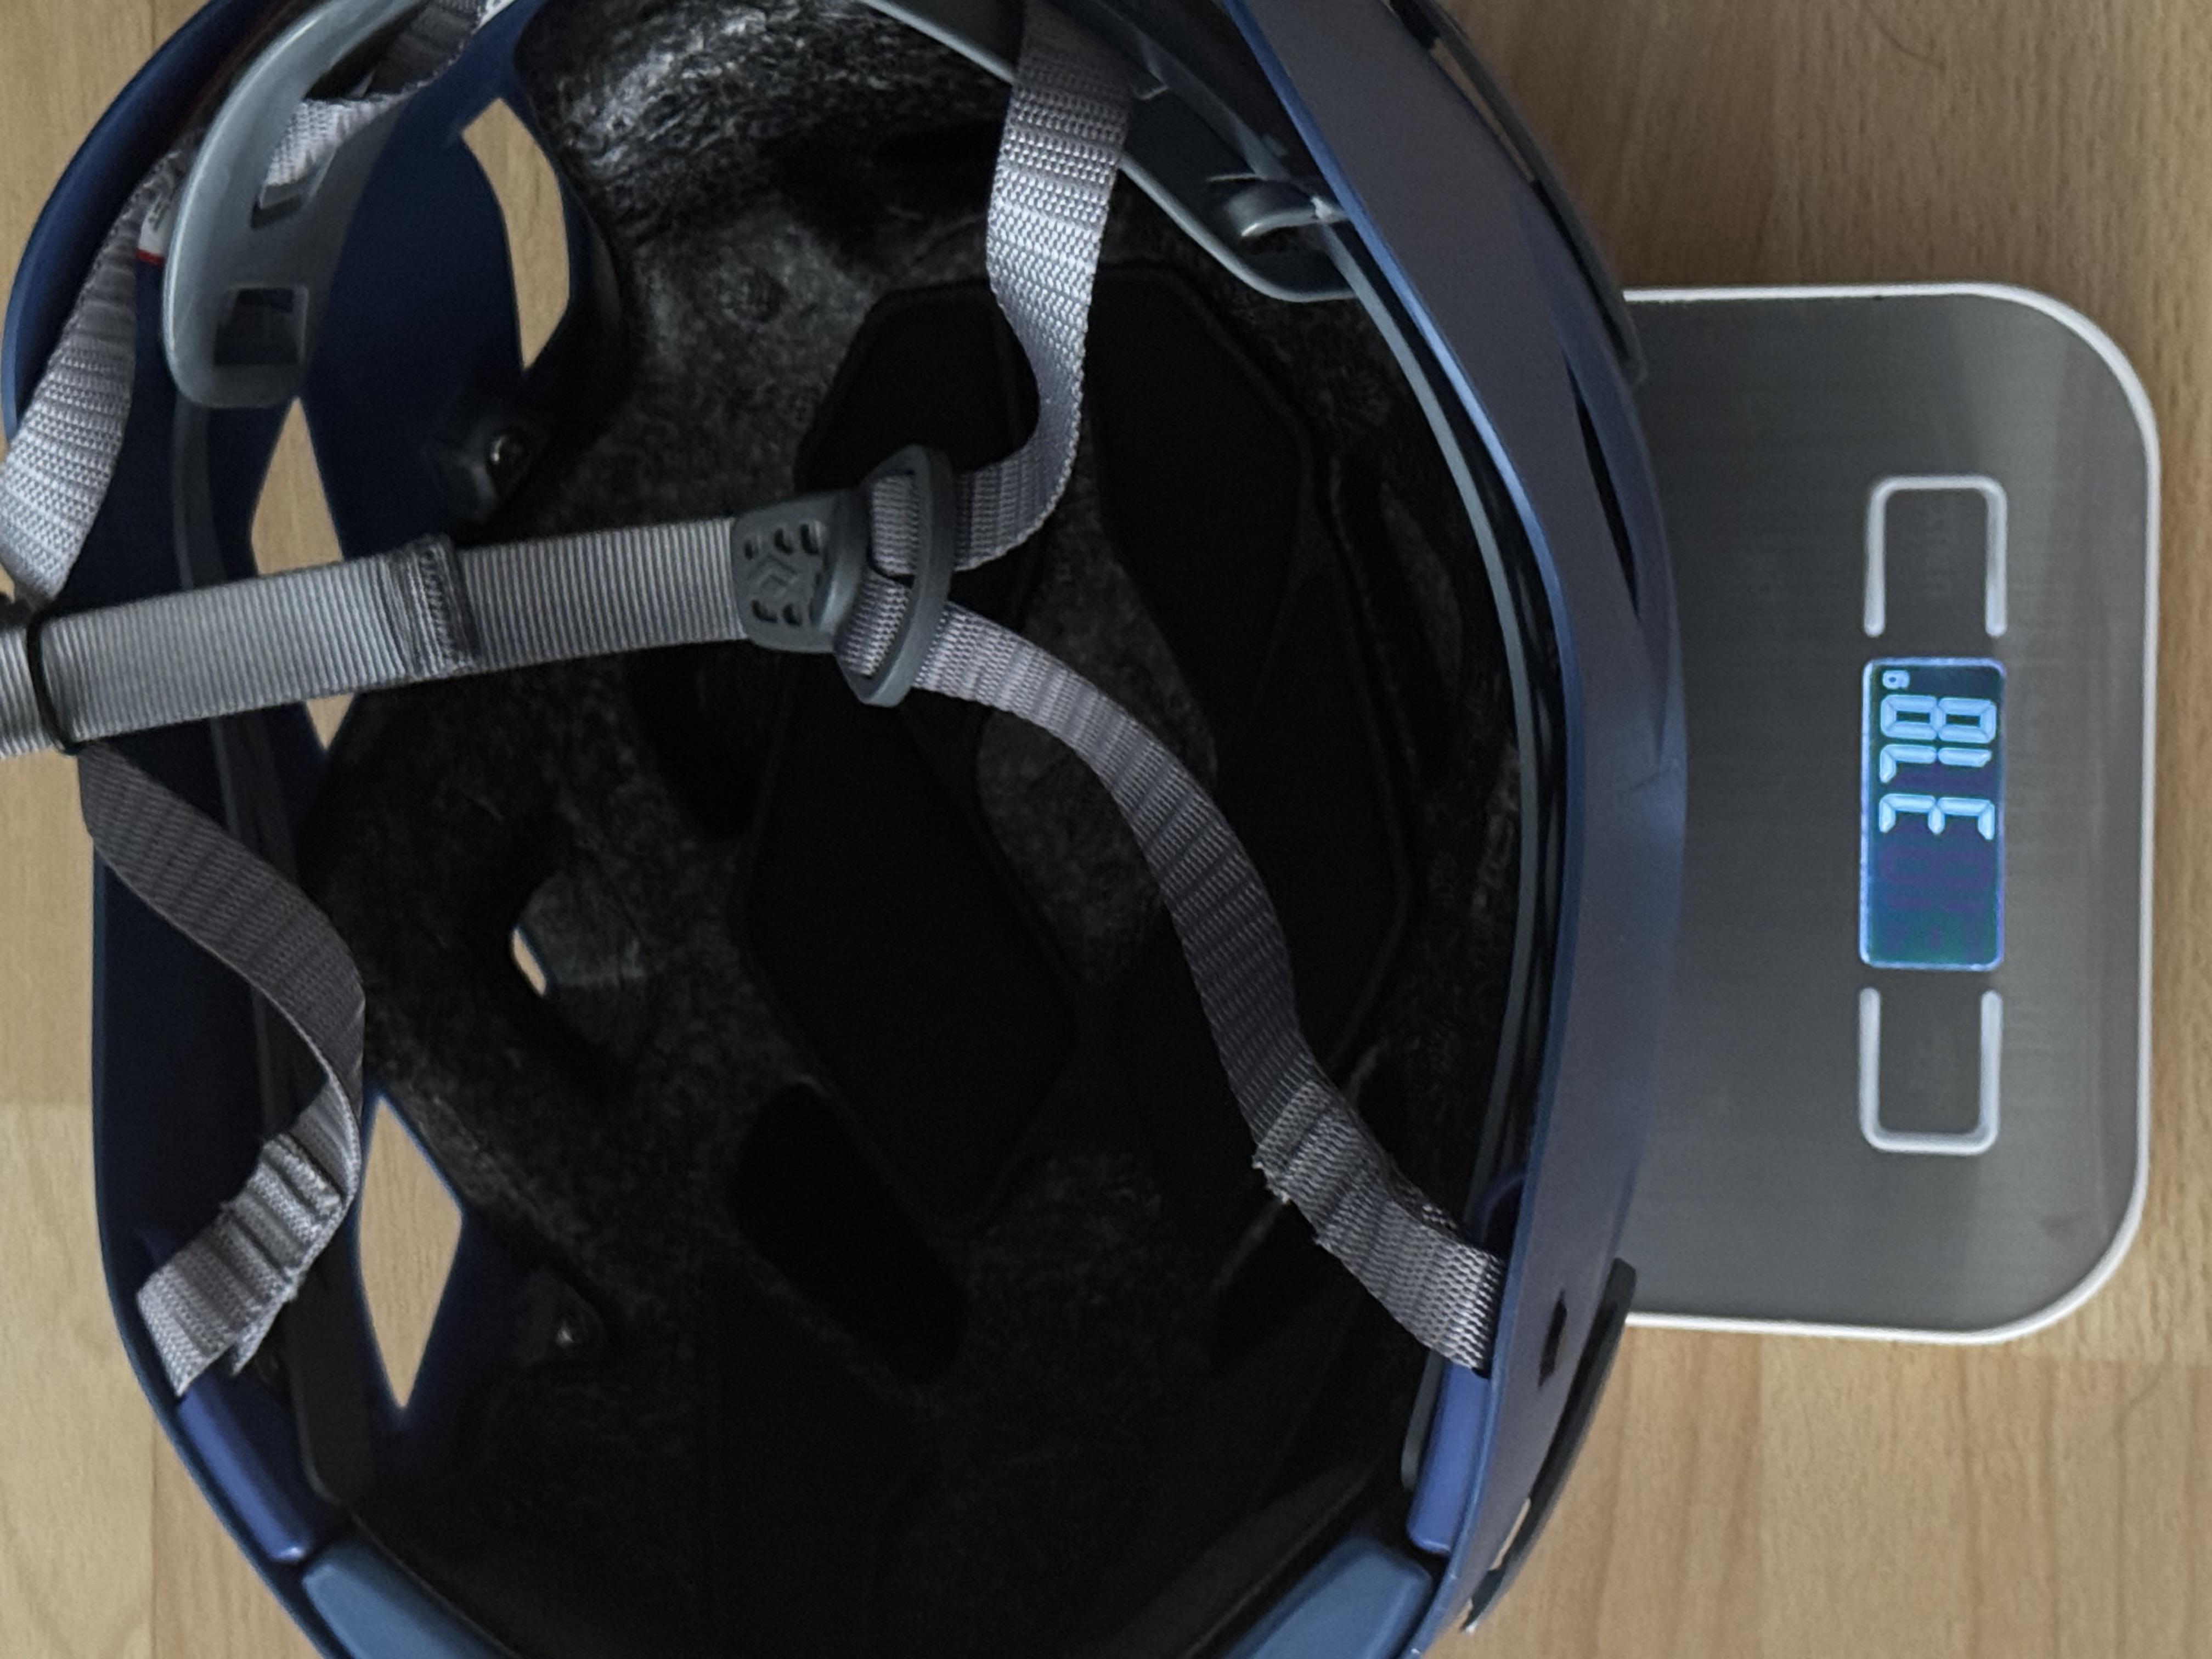
\includegraphics[angle=270,width=\textwidth]{Images/Test_T-RE2-0a}
			\caption*{(a) Test T-RE2-0 (Helmet)}
		\end{minipage}\hfill
		\begin{minipage}{0.48\textwidth}
			\centering
			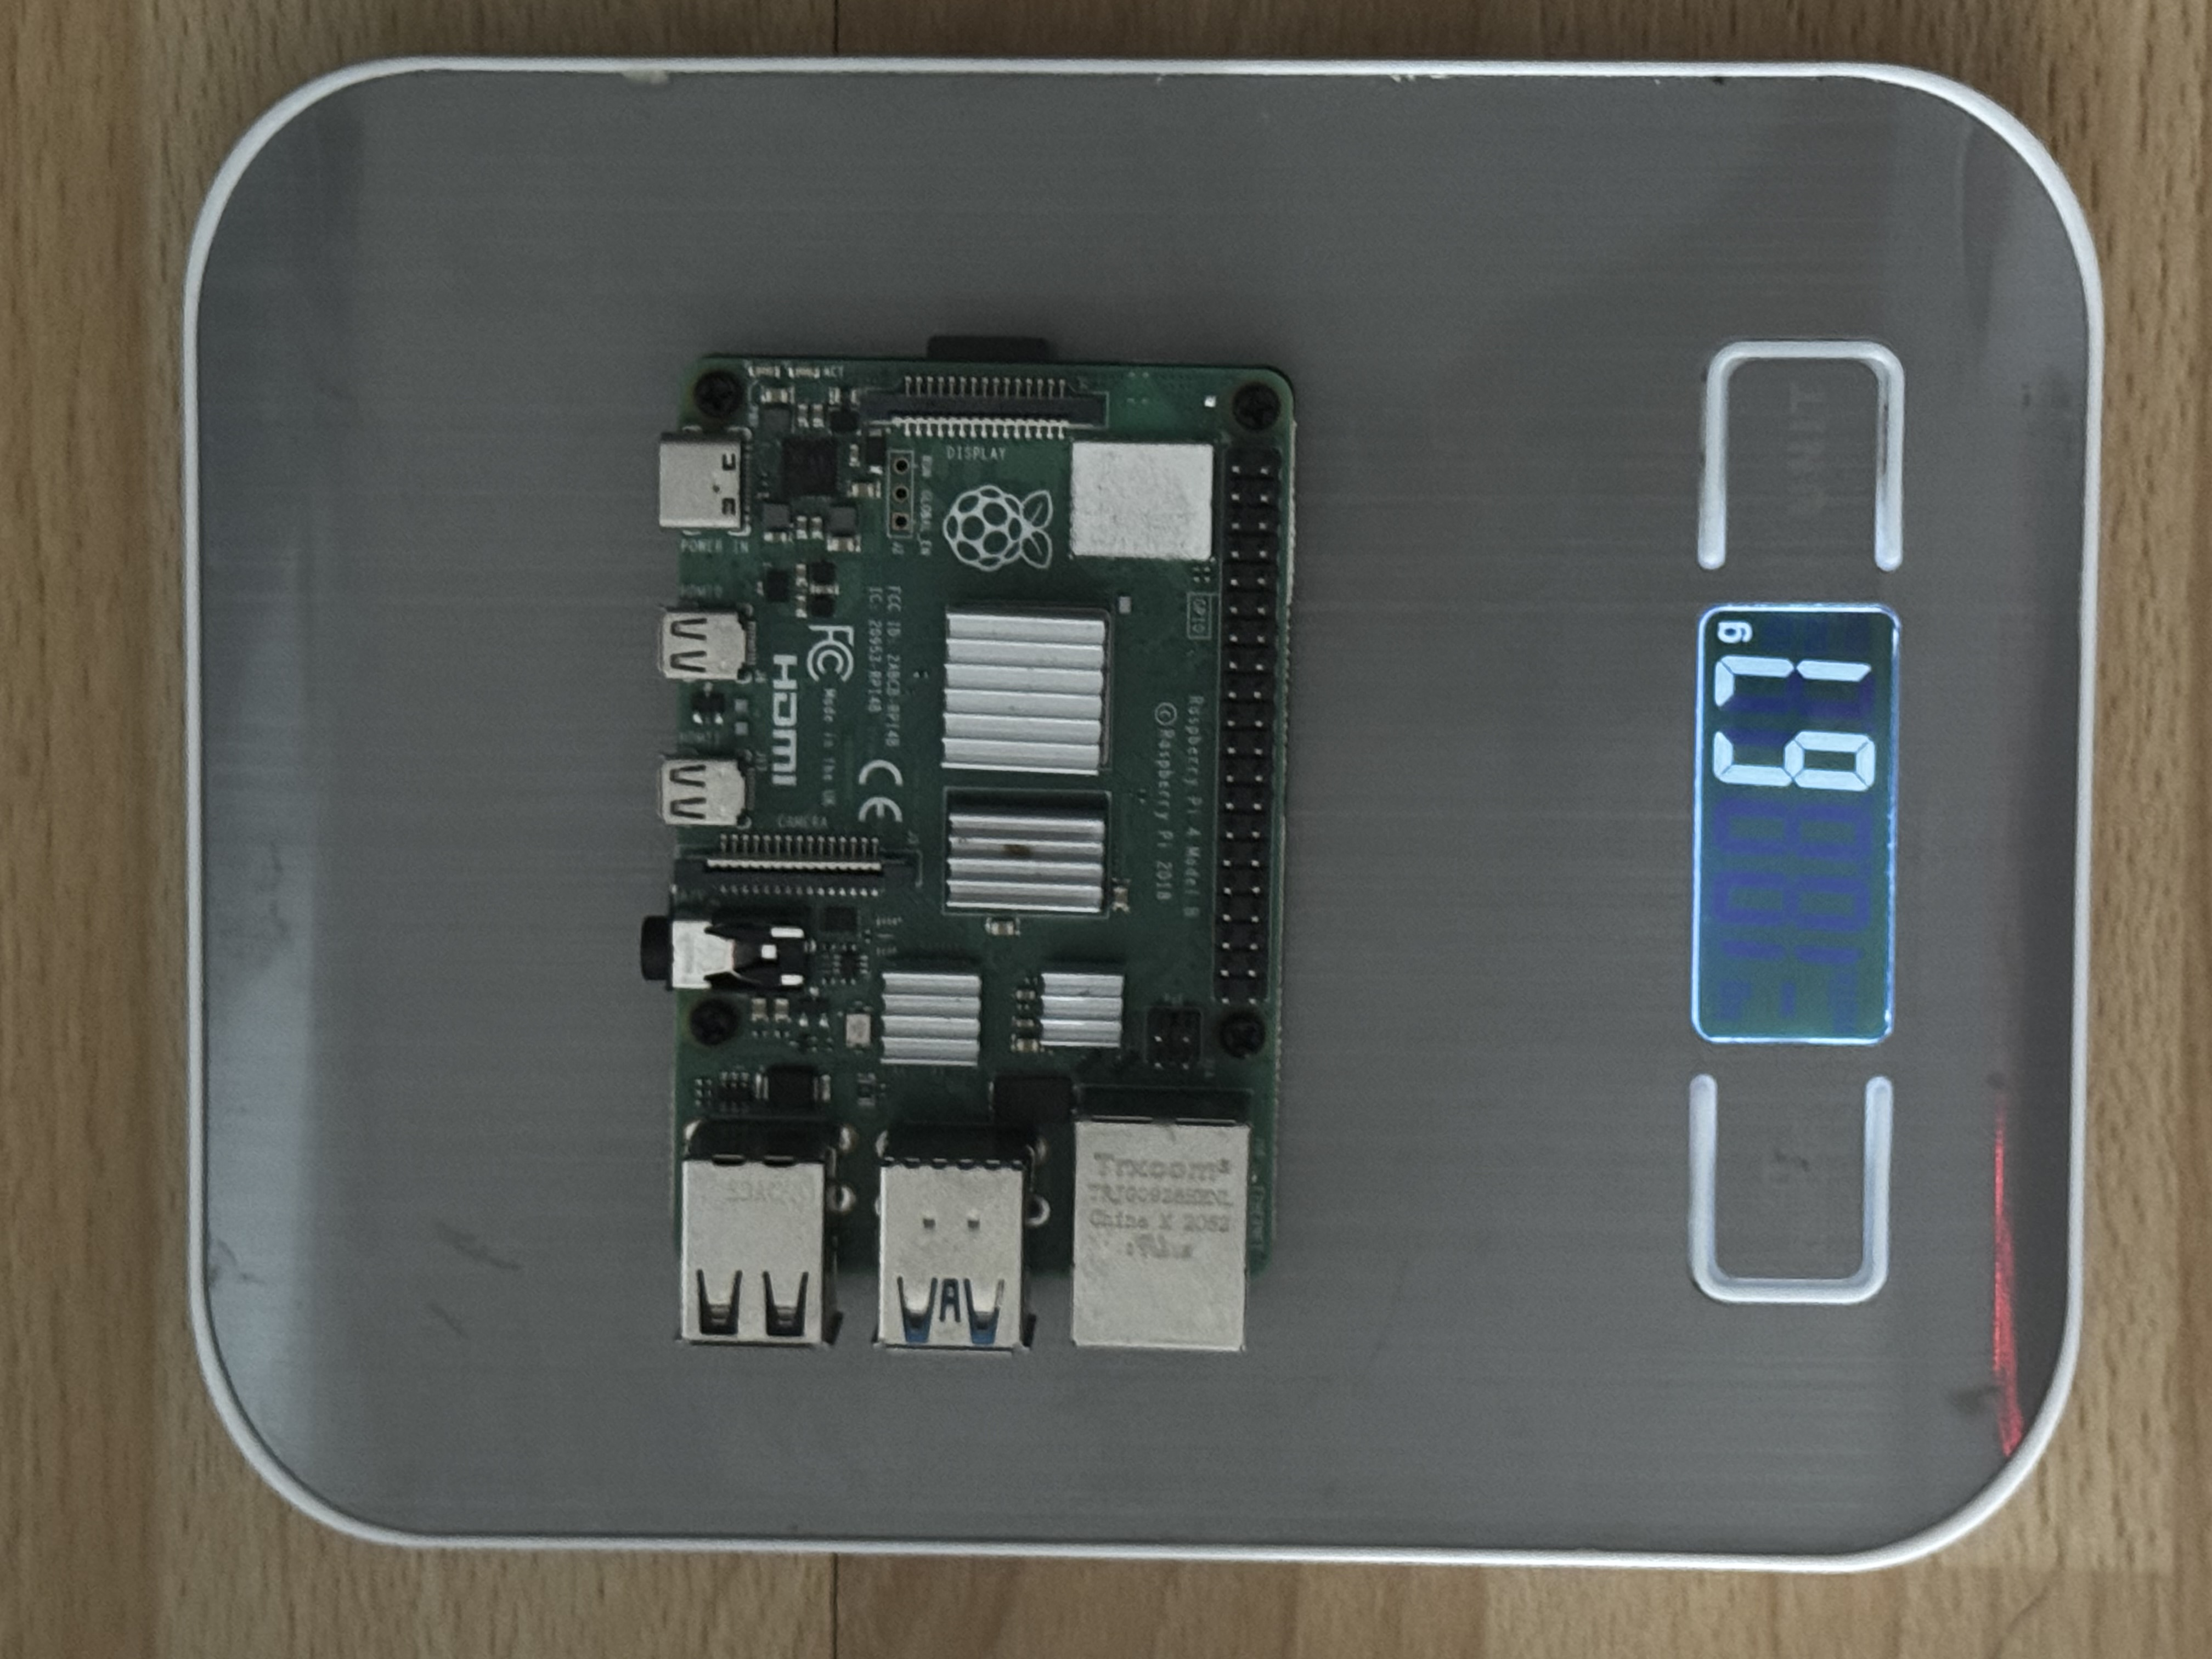
\includegraphics[angle=270,width=\textwidth]{Images/Test_T-RE2-0b}
			\caption*{(b) Test T-RE2-0 (Raspberry Pi 4)}
		\end{minipage}
		\caption{Test T-RE2-0}
	\end{figure}
	
	
	

	
	
\end{document}